\documentclass[11pt,a4paper]{article}
\usepackage[utf8]{inputenc}
\usepackage[portuguese]{babel}
\usepackage[T1]{fontenc}
\usepackage{graphicx}
\usepackage{amsmath}
\usepackage{csquotes}
\usepackage{enumitem}
\usepackage{listings}
\usepackage{xcolor}
\usepackage{eurosym}
\usepackage{hyperref}
\usepackage{biblatex}

\author{Carlos Pinto Machado
	<\href{mailto:cpmachado@protonmail.com}{cpmachado@protonmail.com}>}

\title{Exercícios Resolvidos da AULA AbERTA: Introdução à Estatística}

\addbibresource{./bibliografia.bib}
\makeindex
\lstset{
	language=R,
	basicstyle=\footnotesize,
	numbers=left,
	numberstyle=\tiny\color{gray},
	stepnumber=1,
	numbersep=5pt,
	backgroundcolor=\color{white},
	showspaces=false,
	showstringspaces=false,
	showtabs=false,
	frame=single,
	rulecolor=\color{black},
	tabsize=4,
	captionpos=b,
	breaklines=true,
	breakatwhitespace=false,
	keywordstyle=\color{blue},
	commentstyle=\color{dkgreen},
	escapeinside={\%*}{*)},
	literate=
		{á}{{\'a}}1 {é}{{\'e}}1 {í}{{\'i}}1 {ó}{{\'o}}1 {ú}{{\'u}}1
		{Á}{{\'A}}1 {É}{{\'E}}1 {Í}{{\'I}}1 {Ó}{{\'O}}1 {Ú}{{\'U}}1
		{à}{{\`a}}1 {è}{{\`e}}1 {ì}{{\`i}}1 {ò}{{\`o}}1 {ù}{{\`u}}1
		{À}{{\`A}}1 {È}{{\`E}}1 {Ì}{{\`I}}1 {Ò}{{\`O}}1 {Ù}{{\`U}}1
		{ä}{{\"a}}1 {ë}{{\"e}}1 {ï}{{\"i}}1 {ö}{{\"o}}1 {ü}{{\"u}}1
		{Ä}{{\"A}}1 {Ë}{{\"E}}1 {Ï}{{\"I}}1 {Ö}{{\"O}}1 {Ü}{{\"U}}1
		{â}{{\^a}}1 {ê}{{\^e}}1 {î}{{\^i}}1 {ô}{{\^o}}1 {û}{{\^u}}1
		{Â}{{\^A}}1 {Ê}{{\^E}}1 {Î}{{\^I}}1 {Ô}{{\^O}}1 {Û}{{\^U}}1
		{ã}{{\~a}}1 {ẽ}{{\~e}}1 {ĩ}{{\~i}}1 {õ}{{\~o}}1 {ũ}{{\~u}}1
		{Ã}{{\~A}}1 {Ẽ}{{\~E}}1 {Ĩ}{{\~I}}1 {Õ}{{\~O}}1 {Ũ}{{\~U}}1
		{œ}{{\oe}}1 {Œ}{{\OE}}1 {æ}{{\ae}}1 {Æ}{{\AE}}1 {ß}{{\ss}}1
		{ű}{{\H{u}}}1 {Ű}{{\H{U}}}1 {ő}{{\H{o}}}1 {Ő}{{\H{O}}}1
		{ç}{{\c c}}1 {Ç}{{\c C}}1 {ø}{{\o}}1 {Ø}{{\O}}1 {å}{{\r a}}1 {Å}{{\r A}}1
		{€}{{\euro}}1 {£}{{\pounds}}1 {«}{{\guillemotleft}}1
		{»}{{\guillemotright}}1 {ñ}{{\~n}}1 {Ñ}{{\~N}}1 {¿}{{?`}}1 {¡}{{!`}}1
		{º}{\textdegree}1
}

\begin{document}
\maketitle
\tableofcontents

\clearpage

\section*{Introdução}\addcontentsline{toc}{section}{Introdução}

\paragraph{} No decorrer \cite{OliveiraAulaAberta2017}

\clearpage
\setcounter{section}{3}
\section{Exercícios}
\subsection*{Exercícios Propostos}

\begin{enumerate}[label=\arabic{section}.\arabic*]
	\item \addcontentsline{toc}{subsection}{4.1}
		\begin{enumerate}[label=\alph*)]
		\item $\overline{x} = 19.41667$\hfill
			\lstinputlisting{./recursos/ex4_1a.R}
		\item $s = 1.378954$\hfill
			\lstinputlisting{./recursos/ex4_1b.R}
		\end{enumerate}
	\item \addcontentsline{toc}{subsection}{4.2}\hfill
		\begin{enumerate}[label=\alph*)]
		\item $N = 60$\hfill
			\lstinputlisting{./recursos/ex4_2a.R}
		\item \hfill
			\begin{table}[h!]
				\centering
				\begin{tabular}{|c|c|c|c|}
					\hline
					$x_i$&$n_i$&$N_i$&$f_i$ \\
					\hline
					1000&10&10&0.1666667\\
					\hline
					1100& 8&18&0.1333333\\
					\hline
					1200&12&30&0.2000000\\
					\hline
					1300& 8&38&0.1333333\\
					\hline
					1400&10&48&0.1666667\\
					\hline
					1500&12&60&0.2000000\\
					\hline
				\end{tabular}
			\end{table}
			\lstinputlisting{./recursos/ex4_2b.R}
		\item \hfill
			\begin{align*}
				\overline{x} &= 1260 \\
				s &= 54.09868
			\end{align*}
			\lstinputlisting{./recursos/ex4_2c.R}
		\clearpage
		\item \hfill
			\begin{figure}[h!]
				\centering
				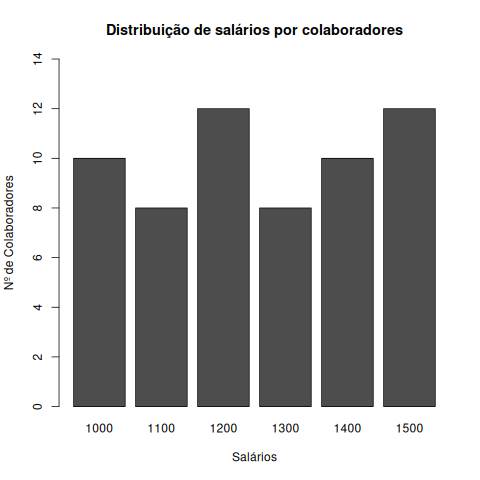
\includegraphics[width=0.7\textwidth]{./recursos/ex4_2d.png}
			\end{figure}
			\lstinputlisting{./recursos/ex4_2d.R}
		\end{enumerate}
	\item \addcontentsline{toc}{subsection}{4.3}\hfill
		\begin{enumerate}[label=\alph*)]
		\item $\overline{x} = 64.26667$\hfill
			\lstinputlisting{./recursos/ex4_3a.R}
		\item $s = 9.676678$\hfill
			\lstinputlisting{./recursos/ex4_3b.R}
		\end{enumerate}
	\clearpage
	\item \addcontentsline{toc}{subsection}{4.4}\hfill
		\begin{enumerate}[label=\alph*)]
		\item \hfill
			\begin{figure}[h!]
				\centering
				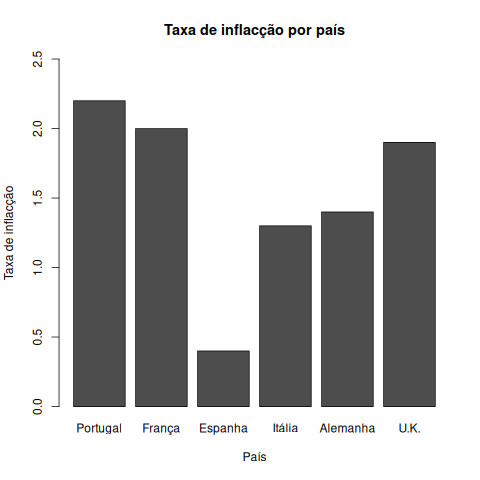
\includegraphics[width=0.7\textwidth]{./recursos/ex4_4a.png}
			\end{figure}
			\lstinputlisting{./recursos/ex4_4a.R}
		\clearpage
		\item \hfill
			\begin{figure}[h!]
				\centering
				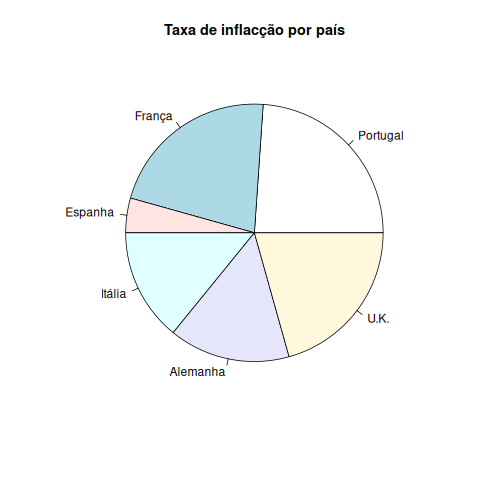
\includegraphics[width=0.7\textwidth]{./recursos/ex4_4b.png}
			\end{figure}
			\lstinputlisting{./recursos/ex4_4b.R}
		\item $\overline{x} = 1.533333$\hfill
			\lstinputlisting{./recursos/ex4_4c.R}
		\end{enumerate}
\end{enumerate}

\printbibliography[heading=bibintoc,title={Bibliografia}]

\end{document}
